%%This is a very basic article template.
%%There is just one section and two subsections.
\documentclass{article}

\usepackage[style=numeric,backend=bibtex]{biblatex}
\usepackage{graphicx}

\bibliography{bib}

\begin{document}


\section*{Dynamic Perfect Hashing - Implementation}

by Lennart Hensler and Frederik Petersen

\section{Introduction}

Dynamic perfect hashing allows for constant find and amortized constant inserts.
We implemented a variant based on \cite{di94}, which uses a two layer approach
to avoid the need of $ n^2 $ space. The outer layer consists of a number of
buckets with a hash function that distributes the data into the buckets. There
may be collisions. Each bucket has its own inner hash function and allows
perfect hashing. If perfect hashing can not be provided in a bucket the data
structure can be resized and/or new hash functions are generated depending on
some conditions.

\section{Parameters}

Several parameters have an impact on the performance and needed space of the
algorithm. We will have a look at several parameters here.

\begin{itemize}
  \item BucketLengthFactor - How much bigger than the desired capacity will a
  bucket be. The smaller this is, the faster the data structure needs to be
  updated. The larger it is, the more space is needed per element.
  \item BucketCapacityFactor - How much bigger than the number of current
  elements will a bucket be created for (capacity-wise).
  \item TODO
\end{itemize}

\section{Experiment Results}

We ran our experiments on a quad core Intel Atom server running a 32bit Debian
Jessie OS with 4GB of RAM. The benchmarks were run automatically each time a
code update was pushed to the repository and plots were generated and saved per
build. That allowed us to test different parameters and compare them to the
earlier builds.

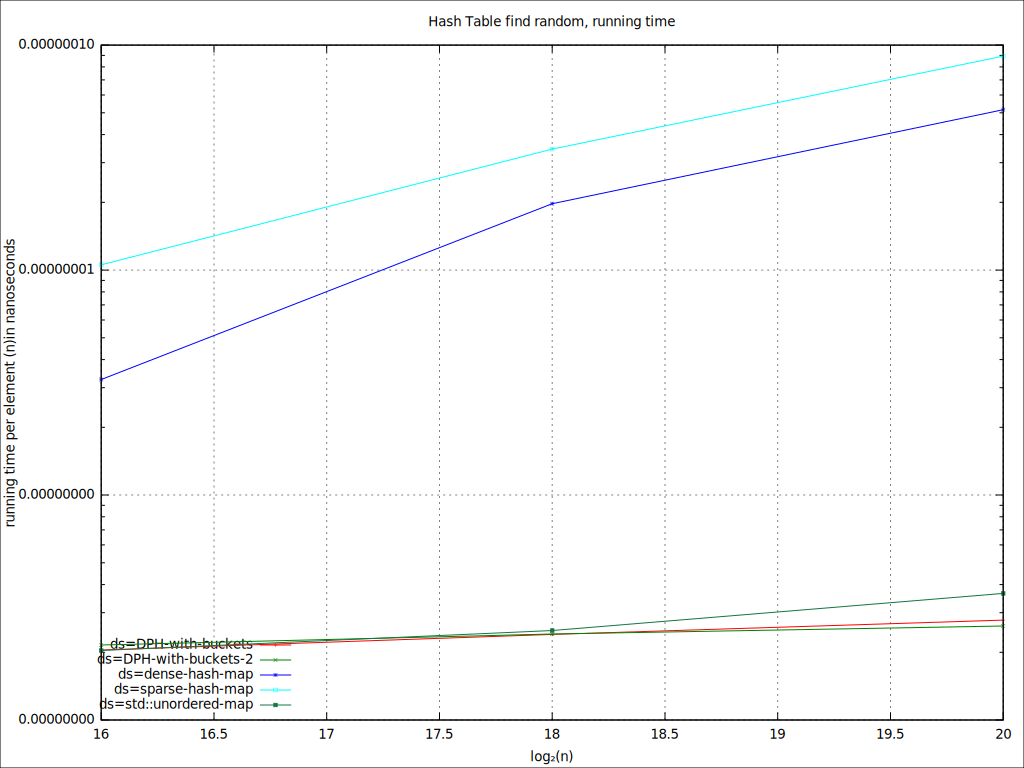
\includegraphics[width=\linewidth]{img/hash_find-random_time}

\section{Further Ideas}

Another approach we tried was having all the buckets in one single array as
described in \cite[p. 94]{mesa08}. We had a lot of issues due to the immense
copying/moving needed, when resizing one of the buckets. This could be avoided
when giving all the buckets some extra space in the array, which they can grow
into without the need to touch other buckets. This, again, would increase the
space requirements.

\printbibliography

\end{document}
